
%% bare_conf.tex
%% V1.3
%% 2007/01/11 
%% by Michael Shell
%% See:
%% http://www.michaelshell.org/
%% for current contact information.
%%
%% This is a skeleton file demonstrating the use of IEEEtran.cls
%% (requires IEEEtran.cls version 1.7 or later) with an IEEE conference paper.
%%
%% Support sites:
%% http://www.michaelshell.org/tex/ieeetran/
%% http://www.ctan.org/tex-archive/macros/latex/contrib/IEEEtran/
%% and
%% http://www.ieee.org/

%%*************************************************************************
%% Legal Notice:
%% This code is offered as-is without any warranty either expressed or
%% implied; without even the implied warranty of MERCHANTABILITY or
%% FITNESS FOR A PARTICULAR PURPOSE! 
%% User assumes all risk.
%% In no event shall IEEE or any contributor to this code be liable for
%% any damages or losses, including, but not limited to, incidental,
%% consequential, or any other damages, resulting from the use or misuse
%% of any information contained here.
%%
%% All comments are the opinions of their respective authors and are not
%% necessarily endorsed by the IEEE.
%%
%% This work is distributed under the LaTeX Project Public License (LPPL)
%% ( http://www.latex-project.org/ ) version 1.3, and may be freely used,
%% distributed and modified. A copy of the LPPL, version 1.3, is included
%% in the base LaTeX documentation of all distributions of LaTeX released
%% 2003/12/01 or later.
%% Retain all contribution notices and credits.
%% ** Modified files should be clearly indicated as such, including  **
%% ** renaming them and changing author support contact information. **
%%
%% File list of work: IEEEtran.cls, IEEEtran_HOWTO.pdf, bare_adv.tex,
%%                    bare_conf.tex, bare_jrnl.tex, bare_jrnl_compsoc.tex
%%*************************************************************************

% *** Authors should verify (and, if needed, correct) their LaTeX system  ***
% *** with the testflow diagnostic prior to trusting their LaTeX platform ***
% *** with production work. IEEE's font choices can trigger bugs that do  ***
% *** not appear when using other class files.                            ***
% The testflow support page is at:
% http://www.michaelshell.org/tex/testflow/


% Note that the a4paper option is mainly intended so that authors in
% countries using A4 can easily print to A4 and see how their papers will
% look in print - the typesetting of the document will not typically be
% affected with changes in paper size (but the bottom and side margins will).
% Use the testflow package mentioned above to verify correct handling of
% both paper sizes by the user's LaTeX system.
%
% Also note that the "draftcls" or "draftclsnofoot", not "draft", option
% should be used if it is desired that the figures are to be displayed in
% draft mode.
%

\begin{filecontents}{bibliography.bib}

@techreport{Symantec-Threat-Report,
    author = "{Symantec}",
    title = {{Internet Security Threat Report (ISTR)}},
    institution = {Symantec Corporation}, 
    year = {2017},
    number = {22}
}

@techreport{IBM-XForce-Report,
    author = "{IBM Security}",
    title = {{IBM X-Force Threat Intelligence Index 2017}},
    institution = {International Buisness Machines},
    year = {2017}
}

@inproceedings{7796146, 
    author={C. DeCusatis and P. Liengtiraphan and A. Sager and M. Pinelli}, 
    booktitle={2016 IEEE International Conference on Smart Cloud (SmartCloud)}, 
    title={Implementing Zero Trust Cloud Networks with Transport Access Control and First Packet Authentication}, 
    year={2016}, 
    pages={5-10}, 
    keywords={authorisation;cloud computing;computer centres;file servers;message authentication;steganography;trusted computing;TCP packet request;authentication token;cloud computing data center;data center security;enterprise-class server;first-packet authentication;steganographic overlay;transport access control;zero trust cloud network;Access control;Authentication;Cloud computing;Logic gates;Servers;authentication;cloud;cybersecurity;token;transport}, 
    doi={10.1109/SmartCloud.2016.22}, 
    month={Nov}
}

@article{GStar,
    author = "{Alan G. Labouseur and Jeremy Birnbaum and Paul W. Olsen, Jr. and Sean R. Spillane and Jayadevan Vijayan and Jeong-Hyon Hwang and Wook-Shin Han}",
    title = {{The G* Graph Database: Efficiently Managing Large Distributed Dynamic Graphs}},
    journal = {Distrib. Parallel Databases},
    issue_date = {December  2015},
    volume = {33},
    number = {4},
    month = dec,
    year = {2015},
    issn = {0926-8782},
    pages = {479--514},
    numpages = {36},
    url = {http://dx.doi.org/10.1007/s10619-014-7140-3},
    doi = {10.1007/s10619-014-7140-3},
    acmid = {2821911},
    publisher = {Kluwer Academic Publishers},
    address = {Hingham, MA, USA},
    keywords = {Big data, Distributed databases, Graphs, Parallel computing, Queries},
}


@misc{REST-API-use,
    author = "{Daniel R. Cogan}",
    title = {{"REpresentational State Transfer in the Modern Internet"}},
    note = {CMC Senior Theses. 1387.},
    howpublished = {\url{http://scholarship.claremont.edu/cmc_theses/1387}},
    year = {2016}
}

@misc{Nissan-Leaf,
    author = "{Troy Hunt}",
    title = {{Controlling vehicle features of Nissan LEAFs across the globe via vulnerable APIs}},
    howpublished = {\url{https://www.troyhunt.com/controlling-vehicle-features-of-nissan/}},
    month = {Feb},
    year = {2016},
    note = {Online, Accessed 7/15/2017}
}

@article{IRS,
    author = "{Stephen Ohlemacher}",
    title = {APNewsBreak: IRS says thieves stole tax info from 100,000},
    journal = {Associated Press},
    month = May,
    year = {2015}
}

@unpublished{honeypot-Def,
    author = "{William W. Martin}",
    title = {{Honey Pots and Honey Nets - Security through Deception}},
    month = {May},
    year = {2001}
}

@book{Stoll:1989:CET:67554,
     author = {Clifford Stoll},
     title = {The Cuckoo's Egg: Tracking a Spy Through the Maze of Computer Espionage},
     year = {1989},
     isbn = {0-385-24946-2},
     publisher = {Doubleday},
     address = {New York, NY, USA}
}

@inproceedings{Provos:2004:VHF:1251375.1251376,
     author = {Niels Provos},
     title = {A Virtual Honeypot Framework},
     booktitle = {Proceedings of the 13th Conference on USENIX Security Symposium - Volume 13},
     series = {SSYM'04},
     year = {2004},
     location = {San Diego, CA},
     pages = {1--1},
     numpages = {1},
     url = {http://dl.acm.org/citation.cfm?id=1251375.1251376},
     acmid = {1251376},
     publisher = {USENIX Association},
     address = {Berkeley, CA, USA}
} 

@book{Graham:2008:FAD:1355323,
     author = {Wayne Graham},
     title = {Facebook API Developers Guide (Firstpress)},
     year = {2008},
     isbn = {1430209690, 9781430209690},
     publisher = {APress}
} 

@inproceedings{SCADA-Testbed-API, 
    author={C. M. Davis and J. E. Tate and H. Okhravi and C. Grier and T. J. Overbye and D. Nicol}, 
    booktitle={2006 38th North American Power Symposium}, 
    title={SCADA Cyber Security Testbed Development}, 
    year={2006}, 
    pages={483-488}, 
    keywords={SCADA systems;power engineering computing;power system control;power system security;public utilities;SCADA cyber security testbed;power system;public networks;public utilities;supervisory control and data acquisition;vulnerability assessment;Access protocols;Communication system control;Computer security;Hardware;IEC standards;Power system modeling;Power system security;Real time systems;SCADA systems;System testing}, 
    doi={10.1109/NAPS.2006.359615}, 
    month={Sept}
}

@misc{Honeypot-API,
    title = {{Http:BL API Specification}},
    howpublsihed = {\url{https://www.projecthoneypot.org/httpbl_api.php}},
    note = {Online, Accessed 7/25/2017}
}

@misc{DoS-Def,
    title = {{Security Tip (ST04-015) Understanding Denial-of-Service Attacks}},
    year = {2013},
    howpublished = {\url{https://www.us-cert.gov/ncas/tips/ST04-015}},
    note = {Online, Accessed 7/15/2017}
}

@article{Hive-Plot,
    author = {Martin Krzywinski and Inanc Birol and Steven Jones JM and Marco A Marra},
    title = {Hive plots—rational approach to visualizing networks},
    journal = {Briefings in Bioinformatics},
    volume = {13},
    number = {5},
    pages = {627-644},
    year = {2012},
    doi = {10.1093/bib/bbr069},
    URL = { + http://dx.doi.org/10.1093/bib/bbr069},
    eprint = {/oup/backfile/content_public/journal/bib/13/5/10.1093/bib/bbr069/2/bbr069.pdf}
}

@misc{XSS-Def,
    title = {{Cross-site Scripting (XSS)}},
    year = {2016},
    note = {Online, Accessed 7/15/2017}
}

@misc{F-Secure,
    author = "{Mikko Hypponen. and Tomi Tuominen.}",
    title = {{F-Secure State of Cyber Security}},
    howpublished = {\url{http://branden.biz/wp-content/uploads/2017/02/cyber-security-report-2017.pdf}},
    Month = {Feb},
    Year = {2017},
    note = {Online, Accessed 7/15/2017}
}

@misc{TheMoon,
    author = "{Bing Liu}",
    title = {{TheMoon - A P2P botnet targeting Home Routers}},
    howpublished = {\url{https://blog.fortinet.com/2016/10/20/themoon-a-p2p-botnet-targeting-home-routers}},
    Month = {Oct},
    Year = {2016},
    note = {Online, Accessed 7/19/2017}
}

@misc{Tomcat-Exploit,
    author = "{Tony Lee}",
    title = {{Manually Exploiting Tomcat Manager}},
    howpublished = {\url{http://blog.opensecurityresearch.com/2012/09/manually-exploiting-tomcat-manager.html}},
    Month = {Sep},
    Year = {2012},
    note = {Online, Accessed 7/19/2017}
}

@misc{Nanohttpd,
    author = "{elonen. and LordFokas. and Richard van Nieuwenhoven.}",
    title = {{NanoHttpd}},
    howpublished = {\url{https://github.com/NanoHttpd/nanohttpd}},
    commit = {f1cb85c},
    year = {2017},
    note = {Online, Accessed 7/15/2017}
}

@misc{unsavoryChar,
    author = "{Lawrence Fernandes}",
    title = {{Shodan: The Hacker’s Search Engine}},
    howpublished = {\url{https://www.cybrary.it/0p3n/intro-shodan-search-engine-hackers/}},
    month = {Mar},
    year = {2016},
    note = {Online, Accessed 7/19/2017}
}

@misc{ab,
    title = {{ab - Apache HTTP server benchmarking tool}},
    howpublished = {\url{https://httpd.apache.org/docs/2.4/programs/ab.html}},
    note = {Online, Accessed 7/15/2017}
}

@misc{3Pillar,
    author = "{Singh Sukhwinder}",
    title = {{Performance Testing of a REstful API using JMeter}},
    howpublished = {\url{https://www.3pillarglobal.com/insights/performance-testing-of-a-restful-api-using-jmeter}},
    note = {Online, Accessed 7/12/2017}
}

@misc{site24x7,
    title = {{Performance Metrics of Rest API Monitor}},
    howpublished = {\url{https://www.site24x7.com/help/performance-metrics/rest-api.html}},
    Month = {Jul},
    Year = {2015},
    note = {Online, Accessed 7/12/2017}
}

@article{performance,
    author = "{Denys Mishunov}",
    title = {{Why Perceived Performance Matters, Part 1: The Perception Of Time}},
    journal = {Smashing Magazine},
    month = {Sep},
    year = {2015},
    note = {Online, Accessed 7/12/2017}
}

\end{filecontents}


\documentclass[10pt, conference]{IEEEtran}
\usepackage{blindtext, graphicx}
% Add the compsoc option for Computer Society conferences.
%
% If IEEEtran.cls has not been installed into the LaTeX system files,
% manually specify the path to it like:
% \documentclass[conference]{../sty/IEEEtran}


% *** CITATION PACKAGES ***
%
\usepackage{cite}
% cite.sty was written by Donald Arseneau
% V1.6 and later of IEEEtran pre-defines the format of the cite.sty package
% \cite{} output to follow that of IEEE. Loading the cite package will
% result in citation numbers being automatically sorted and properly
% "compressed/ranged". e.g., [1], [9], [2], [7], [5], [6] without using
% cite.sty will become [1], [2], [5]--[7], [9] using cite.sty. cite.sty's
% \cite will automatically add leading space, if needed. Use cite.sty's
% noadjust option (cite.sty V3.8 and later) if you want to turn this off.
% cite.sty is already installed on most LaTeX systems. Be sure and use
% version 4.0 (2003-05-27) and later if using hyperref.sty. cite.sty does
% not currently provide for hyperlinked citations.
% The latest version can be obtained at:
% http://www.ctan.org/tex-archive/macros/latex/contrib/cite/
% The documentation is contained in the cite.sty file itself.


% *** GRAPHICS RELATED PACKAGES ***
%
\ifCLASSINFOpdf
  % \usepackage[pdftex]{graphicx}
  % declare the path(s) where your graphic files are
  % \graphicspath{{../pdf/}{../jpeg/}}
  % and their extensions so you won't have to specify these with
  % every instance of \includegraphics
  % \DeclareGraphicsExtensions{.pdf,.jpeg,.png}
\else
  % or other class option (dvipsone, dvipdf, if not using dvips). graphicx
  % will default to the driver specified in the system graphics.cfg if no
  % driver is specified.
  % \usepackage[dvips]{graphicx}
  % declare the path(s) where your graphic files are
  % \graphicspath{{../eps/}}
  % and their extensions so you won't have to specify these with
  % every instance of \includegraphics
  % \DeclareGraphicsExtensions{.eps}
\fi
% graphicx was written by David Carlisle and Sebastian Rahtz. It is
% required if you want graphics, photos, etc. graphicx.sty is already
% installed on most LaTeX systems. The latest version and documentation can
% be obtained at: 
% http://www.ctan.org/tex-archive/macros/latex/required/graphics/
% Another good source of documentation is "Using Imported Graphics in
% LaTeX2e" by Keith Reckdahl which can be found as epslatex.ps or
% epslatex.pdf at: http://www.ctan.org/tex-archive/info/
%
% latex, and pdflatex in dvi mode, support graphics in encapsulated
% postscript (.eps) format. pdflatex in pdf mode supports graphics
% in .pdf, .jpeg, .png and .mps (metapost) formats. Users should ensure
% that all non-photo figures use a vector format (.eps, .pdf, .mps) and
% not a bitmapped formats (.jpeg, .png). IEEE frowns on bitmapped formats
% which can result in "jaggedy"/blurry rendering of lines and letters as
% well as large increases in file sizes.
%
% You can find documentation about the pdfTeX application at:
% http://www.tug.org/applications/pdftex


% correct bad hyphenation here
\hyphenation{op-tical net-works semi-conduc-tor}
\IEEEoverridecommandlockouts
\usepackage{url}
\begin{document}
%
% paper title
% can use linebreaks \\ within to get better formatting as desired
\title{An API Honeypot for DDoS and XSS Analysis}


% author names and affiliations
% use a multiple column layout for up to three different
% affiliations
\author{\IEEEauthorblockN{G Leaden, Marcus Zimmermann, Casimer DeCusatis, \textit{Fellow, IEEE}, and Alan Labouseur}
\IEEEauthorblockA{School of Computer Science and Mathematics\\
Marist College\\
Poughkeepsie, NY 12601\\
Emails: g.leaden1@marist.edu, marcus.zimmermann1@marist.edu, \\casimer.decusatis@marist.edu, alan.labouseur@marist.edu \thanks{This work was supported by the National Science Foundation under CC*DNI Integration (Area 4): Application Aware Software-Defined Networks for Secure Cloud Services (SecureCloud). Award \#1541384.}}
}


% make the title area
\maketitle


\begin{abstract}
Honeypots are systems built to mimic critical parts of a network, distracting attackers while logging their information to develop attack profiles. This paper discusses the design and implementation of a honeypot disguised as a REpresentational State Transfer (REST) Application Programming Interface (API). This honeypot was deployed as part of the NSF SecureCloud test bed.  We discuss the motivation for this work, design features of the honeypot, and experimental data showing performance under various traffic conditions.  We also present the analysis of both a distributed denial of service (DDoS) attack and a cross-site scripting (XSS) malware insertion against this honeypot.
%\boldmath
%\blindtext[1]
\end{abstract}

\IEEEpeerreviewmaketitle

\section{Introduction}
\label{intro}
In recent years, the number and severity of cyber-attacks has grown significantly \cite{Symantec-Threat-Report, IBM-XForce-Report}, \cite{IBM-XForce-Report}. Attackers have managed to pull off massive virtual bank heists, distributed denial of service (DDoS) attacks powered by botnets of the Internet of Things (IoT) devices, and even malware-cause power outages \cite{IBM-XForce-Report}. The National Science Foundation (NSF) SecureCloud test bed aims to combat the growing number of cyber-attacks against cloud networks using an autonomic, zero trust environment \cite{7796146}.  Our most recent implementation utilizes new software developed for use in an Observe Orient Decide Act (OODA) control plane.

Part of this system uses the GStar graph database application to collect and analyze data. Specifically, GStar makes use of a PostGreSQL object relational database, which allows us to perform mathematical analysis on cyber-attack data \cite{GStar}.  After making our initial work available online, we observed a number of unauthorized connection attempts against the GStar Application Programming Interface (API).  More specifically, the attacks targeted GStar's REpresentational State Transfer (REST) API, which is among the most commonly used API architectures \cite{REST-API-use}. There are many examples of recent attacks against REST APIs, including well publicized attacks on the Nissan Leaf smart car \cite{Nissan-Leaf} and the Internal Revenue Service database \cite{IRS}.  Existing APIs often do not follow security best practices, and developers can be lulled into a false sense of security believing that the API will not be an attack target.  Given the recent unsolicited attacks against GStar, we felt it was appropriate to create a more structured profile of these attacks, in an effort to improve the security of our system and other REST APIs.

To accomplish this, we created a low-interaction API honeypot to collect data on these attacks.  Honeypots are servers or systems built and deployed to mimic critical parts of a network, effectively distracting attackers and logging attack information in the process \cite{honeypot-Def}. Disguising a honeypot as an API allows us to analyze and understand attack patterns.  Since our defensive response improves as we collect more data, we can effectively use the attackers' strengths against them; the more times our honeypot is attacked, the better our defense posture becomes.  Since our original REST API was not designed to comprehensively log attack data, we only captured the timestamp, source, command type, and command text for the initial attacks.  To address these shortcomings, we created a new API honeypot, aptly named Pasithea (the Greek goddess of rest), capable of creating an attack profile that includes the user agent, the IP address, and other the information extracted from GStar.

The information gathered from Pasithea can help us determine where attacks are coming from, how they can be classified, and what can be done to defend against such attacks.  Our API honeypot Pasithea has been deployed online, and data collected from this and other sources will be integrated into the NSF SecureCloud test bed project.  Our honeypot enables security experts to analyze and remedy emerging attacks, to avoid falling into framework-complacency.  While various types of honeypots have existed for some time \cite{Stoll:1989:CET:67554}, \cite{Provos:2004:VHF:1251375.1251376}, and many security projects use APIs to make their data more easily consumable \cite{Graham:2008:FAD:1355323},\cite{SCADA-Testbed-API}, the use of a REST API itself to attract malicious traffic and collect attack data does not appear to have been studied previously.  It is important to note a potential source of confusion regarding API honeypots. Honeypot APIs, though similar in name, are not to be confused with Pasithea, which is an API honeypot. A honeypot API is an API made to interface with a specific honeypot, returning useful data or executing certain methods specified by the request \cite{Honeypot-API}. An API honeypot such as Pasithea, on the other hand, is entirely different; it functions as a proper honeypot by gathering data on unauthorized API requests.  This type of API honeypot represents a novel approach to attack analysis that will hopefully lead to the development of more secure and robust APIs for cloud-based applications.

The remainder of this paper is organized as follows. Section II presents the analysis of the data received from both the GStar REST API logs and current data collected by Pasithea. Section III describes the software design and features of Pasithea. Lastly, Section IV presents the results from performance testing against Pasithea.


\section{Analysis}
\label{Analysis}
Pasithea is intended to help investigate multiple types of attacks.  In particular, we observed and analyzed a distributed denial of service (DDoS) flood and the attempted use of cross-site scripting (XSS) commands. In a DDoS attack, an attacker floods a network or service with information or requests in an attempt to exhaust some finite system resource such as memory \cite{DoS-Def}. The goal of a DDoS attack varies, but it is most commonly intended to disrupt legitimate users from accessing information or services provided by the network.

The DDoS attack on GStar lasted from May 25, 2017 until June 01, 2017, creating over 275,000,000 log entries. During this time, the requests per second (R/s) steadily rose, starting at 500 R/s and peaking at over 6000 R/s. Perhaps as an unintended side effect, the log file grew to over 18,022,141,952 bytes (18 Gigabytes) until the GStar Graph Database ran out of storage on its cloud hosted server. The requests received during the DDoS attack all contained the command type HEAD and the command text 'home'.

We gathered a simple random sample of 150 requests collected by the GStar logs between February 06, 2017 and May 25, 2017.  This data was then inserted into a hive plot to visualize and better interpret the attack. Hive plots are a perceptually uniform, scalable visualization for network analytics \cite{Hive-Plot}.  We use a four axis graph to visualize the relationships between timestamp, data source, command type, and response message (as shown in Fig. 1). The timestamp axis is the most heavily populated, containing distinct plotted points for each second during which a log entry was created. The source and message axes are closely related because there is only one plotted point on each axis. Source is the source of the response or message returned by the GStar Graph Database, and message is the response itself. In the context of the log file analyzed, the source is always 'back-end' and message is always 'Unknown command:'. Lastly, the plotted points on the command type axis delineate unique HTTP request methods such as GET, POST, HEAD, PUT, DELETE, etc.

Fig. \ref{fig:regHive} displays all 150 requests, while Fig. \ref{fig:uniqHive} highlights the outlying requests from Fig. \ref{fig:regHive} that did not use the command type GET.  Rather, these requests used the command types POST and HEAD. The POST requests are shown as the plotted point second closest to the center of the axis, while the HEAD requests are the farthest plotted point from the center of the axis. Fig. \ref{fig:uniqHive} represents requests that used methods not commonly employed by web browsers or web crawlers, the two most frequent sources of unwanted requests found in data gathered by Pasithea. This suggests these requests were deliberate and potentially malicious in nature.

Cross-site scripting attacks are a type of injection where malicious scripts are injected into an otherwise benign or trusted website \cite{XSS-def}. Further investigation of the specific commands being attempted as an XSS attack revealed the following:

\noindent GET cgi\\
POST command.php\\
GET ;rm\$IFS-f\$IFS’\\
GET ;wget\$IFS-O\$IFS’\\
GET ;chmod\$IFS’777’\$IFS’\\
GET ;sh\$IFS-c\$IFS‘

\begin{figure}[h]
\centering
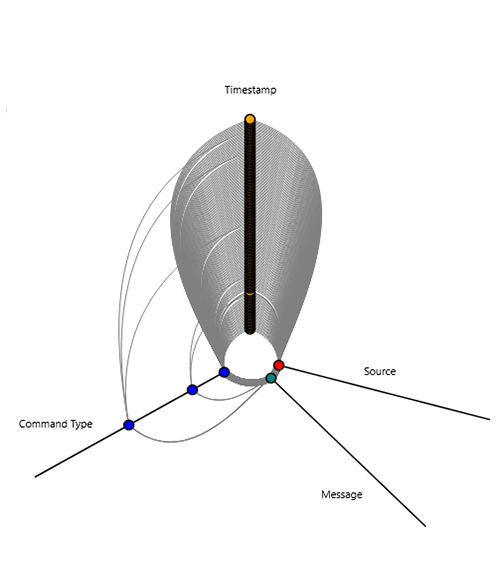
\includegraphics[width=2.5in]{images/regHive.png} 
\caption{-- Hive plot displaying a simple random sample of 150 points from the GStar Graph Database logs. Data sampled is from Feb 06, 2017 - May 25, 2017}
\label{fig:regHive}
\end{figure}

\begin{figure}[h]
\centering
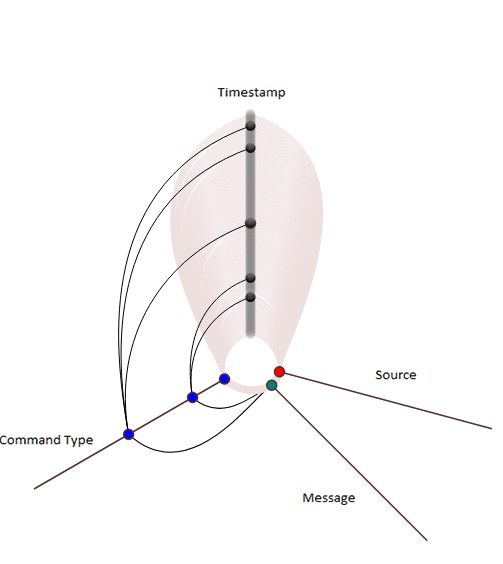
\includegraphics[width=2.5in]{images/uniqHive.png} 
\caption{-- Hive plot where the prominent nodes in the figure denote 'injections' into the GStar Graph Database that differ from normal traffic. Data sampled is from Feb 06, 2017 - May 25, 2017}
\label{fig:uniqHive}
\end{figure}

\noindent Fig. \ref{fig:XSS} displays a selected sample collected by the GStar logs between March 11, 2017 and March 16, 2017 in a hive plot. The highlighted requests range a span of 25 seconds where the XSS commands were attempted, starting with GET cgi and ending with GET ;sh\$IFS-c\$IFS'. This shows both the short amount of time it took to run this malware insertion, and the use of GET and POST request methods for one attack.

\begin{figure}[h]
\centering
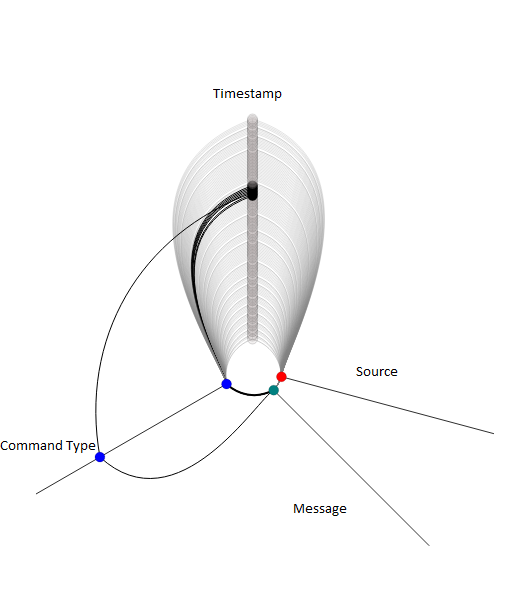
\includegraphics[width=2.5in]{images/XSS.png} 
\caption{-- Hive plot where the prominent nodes in the figure display the XSS attempt on the GStar Graph Database. Data sampled is from Mar 11, 2017 - Mar 16, 2017}
\label{fig:XSS}
\end{figure}

We determined that a very similar attack sequence was also recently documented by a Finnish cyber-security company named F-Secure \cite{F-Secure}. The commands attempted with the XSS attack are intended to upload a PHP: Hypertext Preprocessor (PHP) file, then send a series of commands that, if executed, would remove a file using the \$IFS variable found in the PHP. Afterwards, it would attempt to download a file with the same variable name and change the permissions on said file so that it can be executed by any user.  Then the attacker subsequently executes the file. Researchers from F-Secure  attribute this attack profile to a Peer to Peer (P2P) botnet named TheMoon \cite{TheMoon}. This example illustrates how we can use data collected from attack attempts to isolate and attribute the attack, provided that we can determine what types of attacks are taking place.

Pasithea was subsequently deployed, and is currently active, on an Amazon Web Services (AWS) EC2 instance in Ashburn, Virginia. Our log files indicate cursory web crawls from Baidu, a Chinese search engine, and some attempts at exploiting a known vulnerability in tomcat web servers using GET /manager/html \cite{Tomcat-Exploit}. We continue to monitor this instance, and additional results will be reported in a future paper.

\section{Construction}
\label{construct}
We constructed Pasithea using Java, a common server side programming language, and NanoHTTPD \cite{Nanohttpd}, a lightweight HTTP library that receives HTTP requests and returns responses.  Implementing this kind of functionality enables Pasithea to simulate a real application server. It accepts any kind of request, regardless of the HTTP method, URL requested, or request body. Pasithea then logs the current time, the HTTP method, the path the client attempted to access, e.g. /index.html, the clients IP address, and the user agent information. Clients always receive a $<$h1$>$404 Not Found$<$/h1$>$ response, regardless of which resource they attempt to access.

We are able to host this honeypot on an AWS EC2 instance using the free micro tier. We chose AWS both because of its appealing free tier model and because we are familiar with the security policies and standards that Amazon sets in place. We modified those default security measures within the AWS instance to enable access to the port hosting the API honeypot. Pasithea is currently indexed on Shodan, a web search engine that indexes Internetconnected devices. Shodan is known for being frequented by the hacker community, making it likely that we will be able to collect additional data \cite{unsavoryChar}.

\section{Performance Tests}
\label{performance}
Performance testing is a critical part of development, so it is important to demonstrate Pasitheas performance under different loads and its ability to log many, potentially thousands, of incoming requests in a short amount of time. In other words, it must respond fast enough to keep malicious users interested while also being stable enough to receive high volumes of incoming requests. To do this, we ran a series of benchmarks using the Apache Bench (ab) tool \cite{ab}. This tool allows us to designate a number of completed requests to be sent to our API honeypot while varying the number of simulated concurrent users. The results from these tests are displayed in Fig. \ref{fig:R/s} and Fig. \ref{fig:T/R}. We researched a baseline response time for a RESTful API to give this data appropriate context. In doing so, we discovered two separate internal tests from software development and web monitoring companies, 3PillarGlobal \cite{3Pillar} and Site24x7 \cite{site24x7}. Paired with some research on the human perception of performance \cite{performance}, we concluded that a 300-ms response time is expected under normal traffic conditions in order for the API honeypot to appear realistic. The data Pasithea collected indicates that we fall well within this range given a concurrency level of 500. In addition, we continued tests at much higher concurrency levels to assess how well Pasithea would perform under extreme stress, like the attempts we saw on the GStar API. Pasithea can, with time, handle a concurrency level over 9000 while still logging more than 90\% of the requests received.

\begin{figure}[ht]
\centering
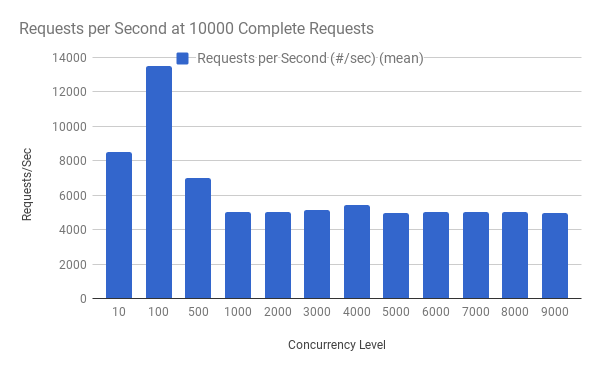
\includegraphics[width=2.5in]{images/RequestsperSecond.png} 
\caption{-- Requests processed per second by Pasithea at varying concurrency levels.}
\label{fig:R/s}
\end{figure}

\begin{figure}[ht]
\centering
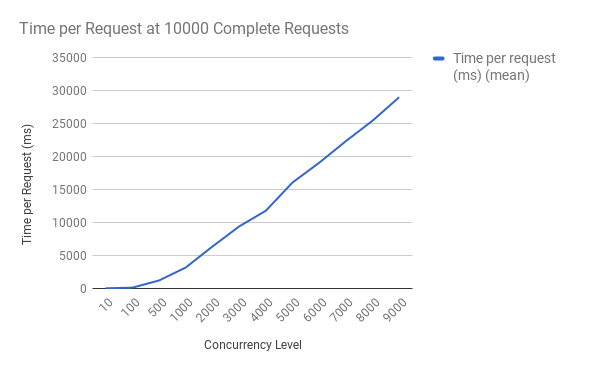
\includegraphics[width=2.5in]{images/TimeperRequest.png} 
\caption{-- Mean time taken to complete a single request on Pasithea at varying concurrency levels.}
\label{fig:T/R}
\end{figure}

Since our implementation of request/response for Pasithea was deliberately kept very simple (only responding with 404 errors), we have thus far been unsuccessful in driving Pasithea hard enough during performance testing to reach a point where it is unable to handle a significant amount of requests.  Pasithea hits a R/s plateau at a concurrency level of 1000, but continues to perform well at 9000. With enough storage space, we believe that Pasithea could withstand a substantial attack, such as the one seen on the GStar Graph Database, and be able to log information about the attack for further analysis.

\section{Conclusion}
\label{conclusion}
The API security landscape resembles more of a Wild West of missing standards, rather than a safe, civilized, city of consistency. This has led to an influx of attacks directed at APIs on many  fronts. Based on the attacks targeting the GStar Graph Database and our research into related attacks, we have constructed an API honeypot, Pasithea, with Java and NanoHTTPD to help combat and detail future attacks on the API landscape. Using hive plots and other tools, we have analyzed a real-world attack on the GStar database, demonstrating how DDoS and XSS attacks can be uncovered and attributed so that a proportionate defense may be deployed.  Our performance data suggests that Pasithea should be able to keep a malicious user interested with fast response times, while also maintaining composure and stability under high traffic loads. This allows us to develop accurate API attack profiles which will help shape the future of API security.

% use section* for acknowledgement
\section*{Acknowledgment}
\label{Acknowledgements}
The authors would like to thank D. Eidle and T. Famularo for their contribution in analyzing the data gathered from the GStar Graph Database.  M. A. Hoffmann and J. Heiles for reviewing the paper and giving their thoughts from an outside perspective. And T. Magnusson for his help constructing Pasithea, as well as reviewing and suggesting edits to the many drafts of this paper.


% Can use something like this to put references on a page
% by themselves when using endfloat and the captionsoff option.
\ifCLASSOPTIONcaptionsoff
  \newpage
\fi


% references section

% can use a bibliography generated by BibTeX as a .bbl file
% BibTeX documentation can be easily obtained at:
% http://www.ctan.org/tex-archive/biblio/bibtex/contrib/doc/
% The IEEEtran BibTeX style support page is at:
% http://www.michaelshell.org/tex/ieeetran/bibtex/
%\bibliographystyle{IEEEtran}
% argument is your BibTeX string definitions and bibliography database(s)
%\bibliography{IEEEabrv,../bib/paper}
%
% <OR> manually copy in the resultant .bbl file
% set second argument of \begin to the number of references
% (used to reserve space for the reference number labels box)
\bibliographystyle{ieeetran}
\bibliography{bibliography}{}


% biography section
% 
% If you have an EPS/PDF photo (graphicx package needed) extra braces are
% needed around the contents of the optional argument to biography to prevent
% the LaTeX parser from getting confused when it sees the complicated
% \includegraphics command within an optional argument. (You could create
% your own custom macro containing the \includegraphics command to make things
% simpler here.)
%\begin{biography}[{\includegraphics[width=1in,height=1.25in,clip,keepaspectratio]{mshell}}]{Michael Shell}
% or if you just want to reserve a space for a photo:


%\begin{IEEEbiography}[{\includegraphics[width=1in,height=1.25in,clip,keepaspectratio]{picture}}]{John %Doe}
%\blindtext
%\end{IEEEbiography}


% You can push biographies down or up by placing
% a \vfill before or after them. The appropriate
% use of \vfill depends on what kind of text is
% on the last page and whether or not the columns
% are being equalized.


%\vfill


% Can be used to pull up biographies so that the bottom of the last one
% is flush with the other column.
%\enlargethispage{-5in}
% that's all folks
\end{document}

